% Relazione project work - Network and Cloud Infrastructures, A.A. 2025/26
% Compilatore: pdfLaTeX (default di Overleaf).
% Frontespizio: modello UNINA, loghi in img/logo/.
\documentclass[11pt,a4paper]{article}

\usepackage[utf8]{inputenc}
\usepackage[T1]{fontenc}
\IfFileExists{lmodern.sty}{\usepackage{lmodern}}{}
\usepackage[italian]{babel}
\usepackage[a4paper,top=2.2cm,bottom=2.2cm,left=2.5cm,right=2.5cm]{geometry}
\usepackage{graphicx}
\usepackage{booktabs}
\usepackage{tabularx}
\usepackage{array}
\usepackage{xcolor}
\usepackage[labelsep=colon,font=small]{caption}
\usepackage{enumitem}
\usepackage{titlesec}
\usepackage{float}
\usepackage{tikz}
\usepackage[hidelinks]{hyperref}

\graphicspath{{figure/}}
\setlist[itemize]{leftmargin=1.4em,itemsep=1pt,topsep=3pt}
\setlist[enumerate]{leftmargin=1.6em,itemsep=1pt,topsep=3pt}
\titleformat{\section}{\large\bfseries}{\thesection}{0.6em}{}
\titleformat{\subsection}{\normalsize\bfseries}{\thesubsection}{0.6em}{}
\titlespacing*{\section}{0pt}{9pt}{4pt}
\titlespacing*{\subsection}{0pt}{6pt}{2pt}
\setlength{\parskip}{3pt}
\setlength{\parindent}{0pt}
\setlength{\textfloatsep}{8pt}
\setlength{\floatsep}{6pt}
\setlength{\intextsep}{6pt}
\renewcommand{\arraystretch}{1.08}
\newcolumntype{Y}{>{\raggedright\arraybackslash}X}
\newcommand{\code}[1]{\texttt{#1}}

\begin{document}

% ------------------------------------------------------------------ copertina
% Frontespizio dal modello UNINA (0_frontespizio.tex), adattato a due candidati.
\begin{titlepage}
\thispagestyle{empty}
\raggedright

\begin{tikzpicture}
\node[anchor=south west] at (4,0) {
\includegraphics[scale=0.75]{img/logo/logo_copertina_1}};
\node[anchor=south west] at (0,1.5) {
\includegraphics{img/logo/logo_copertina_2}};
\node[anchor=south west] at (0,0.5) {\textsf{Scuola Politecnica e delle Scienze di Base}};
\node[anchor=south west] at (0,0) {\textsf{Corso di Laurea Magistrale in Ingegneria Informatica}};
\end{tikzpicture}

\vfill

{\large Elaborato finale in \textbf{Networks and Cloud Infrastructures}}
\\[1cm]
{\textbf{\textit{\LARGE Rilevamento e mitigazione di attacchi DoS in una rete SDN}}}
\\[1cm]
{\large Anno Accademico 2025/2026}

\vfill

{\raggedright Candidati}\\[2pt]
\begin{tabular}{@{}l@{\hspace{1.5em}}l@{}}
\textbf{Massimo Marrone} & \textbf{matr. M63006784}\\
\textbf{Carmine Bellotti} & \textbf{matr. M63001742}\\
\end{tabular}

\vspace{0.6cm}
{\small Repository: \url{https://github.com/giovannistanco/NCIS_unina/tree/main/2026/Marrone_Bellotti}}

\end{titlepage}
\setcounter{page}{2}

% ------------------------------------------------------------------ testo
\section*{Introduzione}
Nelle reti \emph{Software-Defined Networking} (SDN) il piano di controllo \`e separato dal piano
dati: un controller centrale programma gli switch con regole OpenFlow e ne legge i contatori.
Questa visione globale permette di difendere la rete da un attacco \emph{Denial of Service} (DoS)
in modo selettivo: un attaccante che inonda un collegamento condiviso pu\`o essere isolato senza
penalizzare gli utenti onesti collegati allo stesso switch.

Il progetto realizza su una rete emulata un sistema che \textbf{monitora} il traffico,
\textbf{rileva} gli attacchi e li \textbf{mitiga} bloccando solo il MAC dell'attaccante. Il punto di
partenza \`e il baseline dell'anno precedente, di cui sono stati corretti sei difetti:
over-blocking (blocco della porta intera, ora drop per MAC sorgente), logica tutta nel controller
(ora blocklist condivisa, alimentabile anche dall'esterno), codice monolitico (ora moduli Monitor,
Detector, Mitigator, Blocklist), soglia statica (ora soglia adattiva con tetti assoluti), solo DoS
a rate costante (aggiunto un detector Machine Learning) e topologia banale (ora con un ciclo e due
attaccanti su switch diversi). Ogni scelta \`e verificata con scenari Mininet
ripetibili, con la soglia di successo fissata \emph{prima} di ogni run.

\section{Ambiente di emulazione e strumenti}
\begin{itemize}
  \item \textbf{Docker}: un container Debian 11 (Python 3.9, richiesto da Ryu) con tutte le
        dipendenze a versione fissata, avviato con \code{run.ps1} / \code{run.sh};
  \item \textbf{Mininet} e \textbf{Open vSwitch}: host, switch OpenFlow 1.3 e collegamenti con
        banda e ritardo imposti (\code{TCLink});
  \item \textbf{Ryu}: controller Python che estende lo switch L2 con Spanning Tree
        (\code{simple\_switch\_stp\_13}) con i moduli di difesa;
  \item \textbf{iperf}, \textbf{hping3}: traffico legittimo e flood UDP, SYN, ICMP;
  \item \textbf{scikit-learn}: Random Forest e valutazione del detector ML.
\end{itemize}

\section{Topologia e architettura}
\begin{figure}[H]
  \centering
  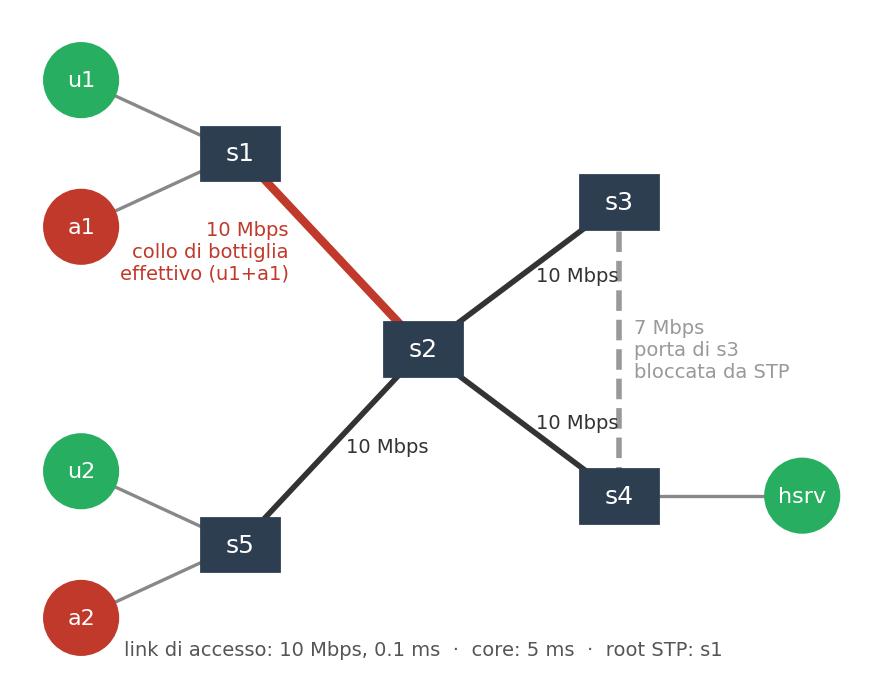
\includegraphics[width=0.42\textwidth]{topology.png}
  \caption{Topologia: 5 switch con ciclo \code{s2--s3--s4--s2}, server \code{hsrv}, utenti
  \code{u1}, \code{u2} e attaccanti \code{a1}, \code{a2}.}
\end{figure}
I collegamenti sono da 10\,Mbps (\code{s3--s4} da 7\,Mbps). Gli attaccanti \code{a1} (su
\code{s1}) e \code{a2} (su \code{s5}) sono su switch diversi; l'utente legittimo \code{u1} \`e sullo
\textbf{stesso switch} di \code{a1}. Dopo la convergenza (circa 35\,s) STP spegne \code{s3--s4} e il
traffico verso il server passa per \code{s1--s2--s4}: il \textbf{collo di bottiglia} \`e l'uplink
\code{s1--s2}, condiviso da \code{u1} e \code{a1}.

Il controller aggiunge allo switch L2 quattro moduli disaccoppiati:
\begin{itemize}
  \item \textbf{Monitor}: ogni 5\,s legge le \emph{flow stats} e calcola per ogni MAC sorgente
        pacchetti/s, byte/s, dimensione media del pacchetto e \textbf{traffico di ritorno}
        (\code{rx}, i pacchetti diretti verso di lei). Le regole di drop sono escluse.
  \item \textbf{Detector} (default: soglia adattiva): media e varianza EWMA su byte/s e pacchetti/s
        per sorgente, pi\`u due \textbf{tetti} che coprono il flood che parte gi\`a al massimo:
        2000\,pps sempre e 0,95\,MB/s solo se la sorgente \textbf{non riceve risposte}
        (\code{rx} $<$ 10\% di quanto manda). Un TCP legittimo riceve ACK (46--100\%), un flood UDP
        no ($\le$ 2\%). Chi riceve pi\`u di quanto manda (il server sotto SYN flood) non viene mai
        segnalato. In alternativa \code{DETECTOR=ml} usa un Random Forest.
  \item \textbf{Conferma 2 su 3}: si blocca dopo 2 intervalli sospetti sugli ultimi 3.
  \item \textbf{Mitigator e Blocklist}: regola OpenFlow di \textbf{drop per MAC sorgente} a
        priorit\`a 100 su tutti gli switch, con scadenza di 60\,s; la whitelist \`e opzionale.
        OVS inoltra al controller al massimo 200 packet-in/s per switch, per proteggere il piano di
        controllo.
\end{itemize}

\section{Funzionamento}
\begin{sloppypar}
Per riprodurre i risultati basta \code{run.sh} (o \code{run.ps1} su Windows), che apre una shell nel
container, e poi \code{bash experiments/run\_all.sh mit}, che esegue da solo la demo; il README del
repository elenca tutti gli scenari e le opzioni. A mano, il sistema si esegue in tre terminali
dentro il container: il controller
(\code{ryu-manager controller.py}, con variabili come \code{WHITELIST=0} o \code{MITIGATE=0}), la
rete (\code{python3 topology.py}) e un terminale di osservazione. Dopo la convergenza di STP,
\code{pingall} conferma la raggiungibilit\`a completa (0\% persi, 20/20). \code{u1} avvia un
download TCP verso \code{hsrv}; poi \code{a1} lancia un flood UDP a 25\,Mbps, oltre il doppio della
capacit\`a dell'uplink:
\end{sloppypar}
\vspace{-2pt}
\begin{center}\small\code{mininet> a1 iperf -c 10.0.0.100 -u -p 5001 -b 25M -t 60 \&}\end{center}
\vspace{-4pt}

Per le figure il controller \`e avviato \textbf{senza whitelist} e con blocco permanente
(\code{WHITELIST=0 BLOCK\_TTL=0}).

\begin{figure}[H]
  \centering
  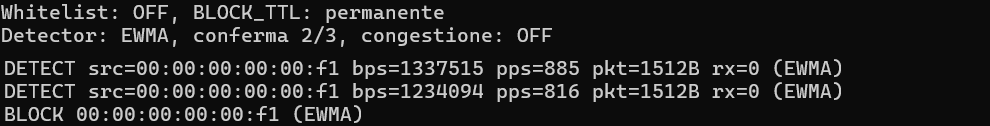
\includegraphics[width=0.66\textwidth]{controller_block.png}
  \caption{Configurazione del controller e rilevamento: due intervalli sospetti
  (\code{rx=0}: a1 non riceve risposte), poi il blocco del MAC di a1 (righe STP omesse).}
\end{figure}

Il controller misura per \code{a1} fino a 1,34\,MB/s, cio\`e l'intero link, con \code{rx=0}: il
primo \code{DETECT} arriva a +5,9\,s dall'inizio del flood, il \code{BLOCK} a +10,9\,s. In
quell'intervallo il download di \code{u1} scende da 9,6 a 4,8\,Mbps e poi quasi a zero; appena
\code{a1} \`e bloccato torna a 9,56\,Mbps e ci resta mentre l'attacco continua (il picco di
23\,Mbps nel secondo successivo al blocco \`e la coda accumulata che si svuota).

\begin{figure}[H]
  \centering
  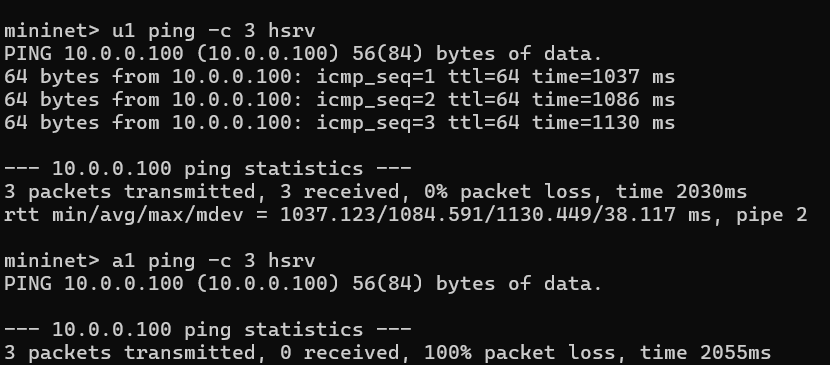
\includegraphics[width=0.5\textwidth]{ping_dopo_block.png}\\[4pt]
  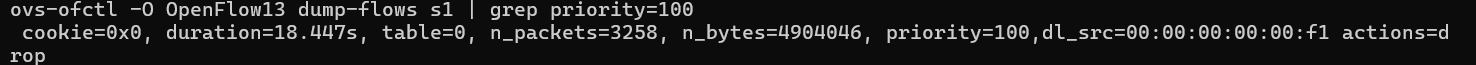
\includegraphics[width=\textwidth]{regola_drop.png}
  \caption{Dopo il \code{BLOCK}: \code{u1} raggiunge il server, \code{a1} perde il 100\% dei ping.
  Sotto, la regola di drop su \code{s1}: priorit\`a 100, \code{dl\_src} di a1, 3258 pacchetti
  del flood scartati in 18\,s.}
\end{figure}

I tempi di risposta di \code{u1} (circa 1\,s) dipendono dal suo stesso download TCP, che riempie
la coda del collegamento; prima dell'attacco, con lo stesso download in corso, erano gi\`a
0,6--0,8\,s, mentre \code{a1} rispondeva in circa 46\,ms.

La stessa scena \`e stata ripetuta in cinque configurazioni (Tabella~\ref{tab:casi}). In tutte
\code{u1} non \`e mai stato segnalato, e prima del flood scaricava a 9,5--9,6\,Mbps.

\begin{table}[H]
\centering\footnotesize
\begin{tabularx}{\textwidth}{@{}Y l c c c@{}}
\toprule
Configurazione & Flood di \code{a1} & DETECT / BLOCK & \code{u1} (10\,s / +20--40\,s) & ping \code{a1} \\
\midrule
Senza mitigazione (\code{MITIGATE=0}) & UDP 25\,Mbps & +5,5\,s / mai & 2,4 / \textbf{1,0}\,Mbps & risponde \\
Con whitelist & UDP 25\,Mbps & +4,6 / +9,6\,s & 1,6 / \textbf{9,6}\,Mbps & 100\% perso \\
Senza whitelist (\code{WHITELIST=0}) & UDP 25\,Mbps & +5,4 / +10,4\,s & 1,4 / \textbf{9,6}\,Mbps & 100\% perso \\
ML (\code{DETECTOR=ml}) & UDP, pacchetti 250\,B & +3,3 / +8,3\,s & 5,4 / \textbf{9,6}\,Mbps & 100\% perso \\
ML (\code{DETECTOR=ml}) & UDP 25\,Mbps & mai / mai & 2,0 / \textbf{0,5}\,Mbps & risponde \\
\bottomrule
\end{tabularx}
\caption{Le cinque casistiche dal vivo: tempi dall'inizio del flood e throughput di \code{u1}.}
\label{tab:casi}
\end{table}

Senza mitigazione il controller vede l'attacco a ogni intervallo ma non interviene, e \code{u1}
resta a 1\,Mbps: un DoS vero e proprio. La soglia adattiva blocca \code{a1} in circa 10\,s con e
senza whitelist. Il ML blocca il flood a pacchetti piccoli anche prima (+8,3\,s), ma non rileva
quello a pacchetti grandi, che ha le stesse feature di un UDP legittimo ad alta banda.

\section{Risultati sperimentali}
Negli scenari automatici (\code{experiments/run\_all.sh}) \code{a1} manda 40\,s di traffico normale
e poi il flood per 60\,s; in \code{cold} il flood parte da subito. Tempi misurati dall'inizio del
flood; con polling a 5\,s e conferma 2/3 il minimo \`e circa 10\,s.

\begin{table}[H]
\centering\small
\begin{tabularx}{\textwidth}{@{}Y Y l@{}}
\toprule
Scenario & Rilevamento e blocco & u1 segnalato \\
\midrule
\code{mit} (whitelist attiva) & a1 bloccato a +9,8\,s & no \\
\code{nowl} (senza whitelist) & a1 bloccato a +9,6\,s & \textbf{no} \\
\code{both}: a1 + a2, senza whitelist, 8 run & entrambi bloccati a +8,8--10,4\,s (8/8) & no \\
\code{cold}, EWMA del baseline & \textbf{mai rilevato} & -- \\
\code{cold}, EWMA + tetti, 6 run & a1 bloccato a +12,2--12,5\,s (6/6) & no \\
SYN flood verso il server, 4 run & a1 bloccato a +9,0--10,2\,s; server mai bloccato & no \\
\bottomrule
\end{tabularx}
\caption{Mitigazione negli scenari automatici.}
\end{table}

\begin{figure}[H]
  \centering
  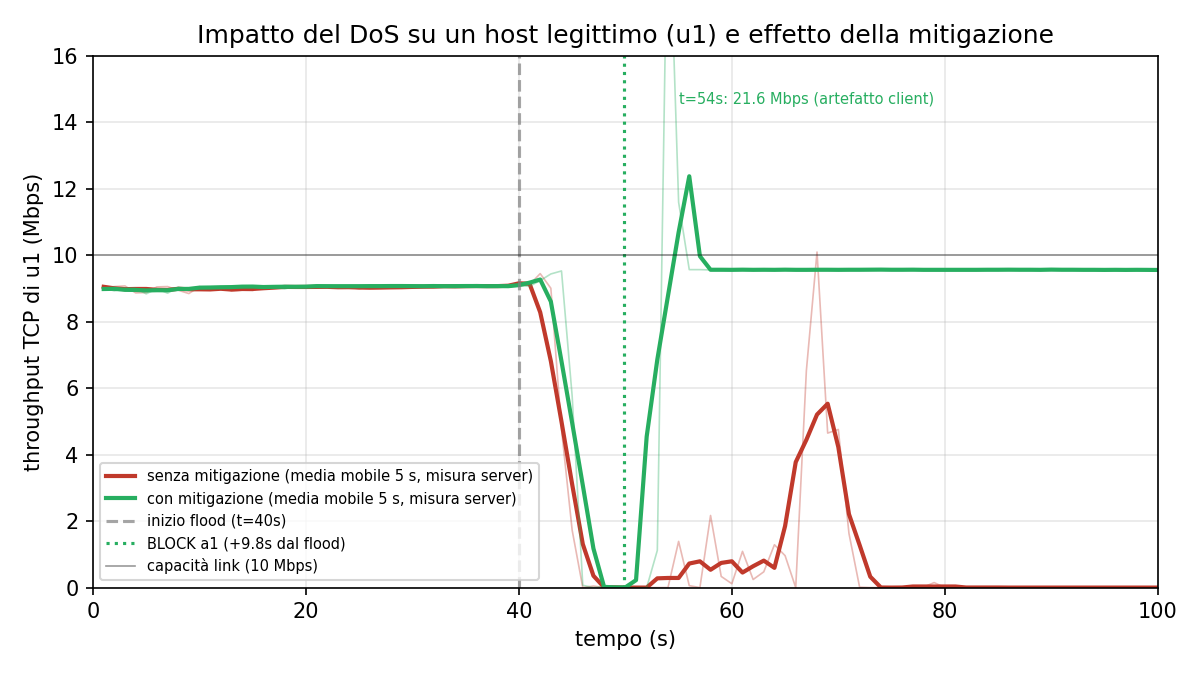
\includegraphics[width=0.62\textwidth]{throughput_compare.png}
  \caption{Throughput TCP di \code{u1}: tra +20 e +60\,s dal flood scende a 2,3\,Mbps senza
  mitigazione e resta a 9,6\,Mbps con la mitigazione (9,0--9,1\,Mbps prima del flood).}
\end{figure}

\textbf{Come ci si \`e arrivati.} Ogni problema \`e stato riprodotto con uno scenario Mininet, corretto e
rimisurato: le regole di drop finivano nelle metriche (escluse); senza whitelist il TCP di
\code{u1}, che satura il link, superava il tetto e veniva bloccato 23,5\,s prima del flood (tetto
solo per chi non riceve risposte); il flood a freddo passava sotto il tetto da 1,1\,MB/s (abbassato
a 0,95); \code{a2} rallentava per un intervallo e ritardava il blocco (isteresi fino a 0,6\,MB/s);
sotto SYN flood le risposte del server sembravano un flood (chi riceve pi\`u di quanto manda non
viene segnalato). Il rilevamento per congestione (\code{CONGESTION=1}) \`e un risultato negativo:
il TCP di \code{u1} porta da solo l'uplink oltre il 90\%, e senza whitelist veniva bloccato
\code{u1}; resta disattivato.

\textbf{Machine Learning.} Dataset generato con \code{gen\_dataset.sh}: 2098 righe, 100 episodi
da 60\,s con traffico benigno vario e attacchi hping3 (UDP, SYN, ICMP, low-rate). La prima
valutazione dava 1,00, ma mescolava campioni dello stesso episodio tra training e test; ora si usa
la \textbf{validazione per gruppo} (episodio e host) e le famiglie SYN e low-rate sono solo di test.

\begin{table}[H]
\centering\small
\begin{tabular}{@{}lccccc@{}}
\toprule
Metodo & Precision & Recall & F1 & FPR & Attaccanti / onesti bloccati \\
\midrule
Random Forest (profondit\`a 4) & 0,39 & 0,95 & 0,55 & 0,21 & 98\% / 19\% \\
Soglia statica (tetti) & 0,33 & 0,57 & 0,42 & 0,17 & 60\% / 18\% \\
EWMA del baseline & 0,00 & 0,00 & 0,00 & 0,01 & 0\% / 2\% \\
EWMA + tetti & 0,32 & 0,65 & 0,43 & 0,20 & 71\% / 21\% \\
\bottomrule
\end{tabular}
\caption{Valutazione offline per campione e per host (conferma 2/3).}
\end{table}

Il ML \`e tenuto come strategia alternativa: i falsi positivi vengono dall'UDP legittimo, che con
le sole feature di flusso ha gli stessi pacchetti/s, byte/s e dimensione di un flood UDP; anche
Gradient Boosting e MLP danno risultati simili, quindi il limite \`e nelle feature. Offline le
soglie sono penalizzate, perch\'e il dataset non registra il traffico di ritorno: in rete la stessa
soglia non ha mai bloccato \code{u1}. Sulla famiglia SYN mai vista il Random Forest prende il 73\%
dei campioni.

\section{Limiti e sviluppi futuri}
\begin{itemize}
  \item Uno streaming UDP legittimo ad alta banda non riceve risposte e supera il tetto: limitarne
        la banda con i \emph{meter} OpenFlow invece di bloccarlo.
  \item Un flood verso un servizio che risponde aggira la regola del traffico di ritorno: feature
        di livello 4 (porte distinte, flag TCP) raccolte con il campionamento \textbf{sFlow} di OVS,
        fuori dal canale OpenFlow per non sovraccaricare il controller.
  \item MAC spoofing: blocco per porta d'ingresso e \emph{port security} sullo switch di accesso.
  \item Circa 10\,s per bloccare e ricadute ogni 60\,s per un attaccante persistente: conferma
        immediata oltre il tetto e durata del blocco crescente.
  \item ML: disattivare l'offload TSO di Mininet, che falsa la dimensione dei pacchetti, e
        aggiungere feature L4.
\end{itemize}

\section{Conclusioni}
Il sistema blocca il flood in circa 10\,s (12\,s se parte a freddo), riporta l'utente legittimo da
2,3 a 9,6\,Mbps e \textbf{non blocca mai il traffico onesto, anche senza whitelist}. L'idea
centrale \`e semplice e verificabile: un flood manda tanto e non riceve niente. Codice, log e
istruzioni di riproduzione sono nel repository
\url{https://github.com/giovannistanco/NCIS_unina/tree/main/2026/Marrone_Bellotti}.

\end{document}
